% !TeX spellcheck = en_US
\addsection{Recommendations}{\art/haste.png}

\iftoggle{printable}{}{\bigbreak}

\begin{multicols}{2}
We've gathered up some custom rules and best practices to make your gaming experience as smooth as possible.
Bear in mind that those are just \textbf{opinions of the authors} of this book.
Enjoy.

\subsection*{Play Time}

You can estimate your \textbf{minimal} play time using the following formula:

\begin{center}
  Play Time $= \boldsymbol{P × R × 5}$ [min]
\end{center}

Where:
\begin{itemize}
  \item[$\textbf{P}$] -- number of players
  \item[$\textbf{R}$] -- number of rounds
\end{itemize}

Therefore, if you're playing a 3-player scenario consisting of 12 rounds, you can easily calculate that $3 × 12 × 5 = 180$.
Your expected minimal play time should be around 3 hours.
To calculate the \textbf{upper bound} of your play time (more realistic if there are inexperienced players), just double the result.
So in this case that would be 6 hours.

\subsection*{Magic Arrows}

Except for the Magic Arrow, every spell appears exactly twice in the spell deck.
After players prepare their starting M\&M decks, it is recommended to remove as many Magic Arrows from the spell deck, so that at most two of them remain.

\subsection*{Trading Post}

Although rules as written state that you can remove only one card from your hand while visiting a Trading Post, it is recommended to allow removing as many as you like.

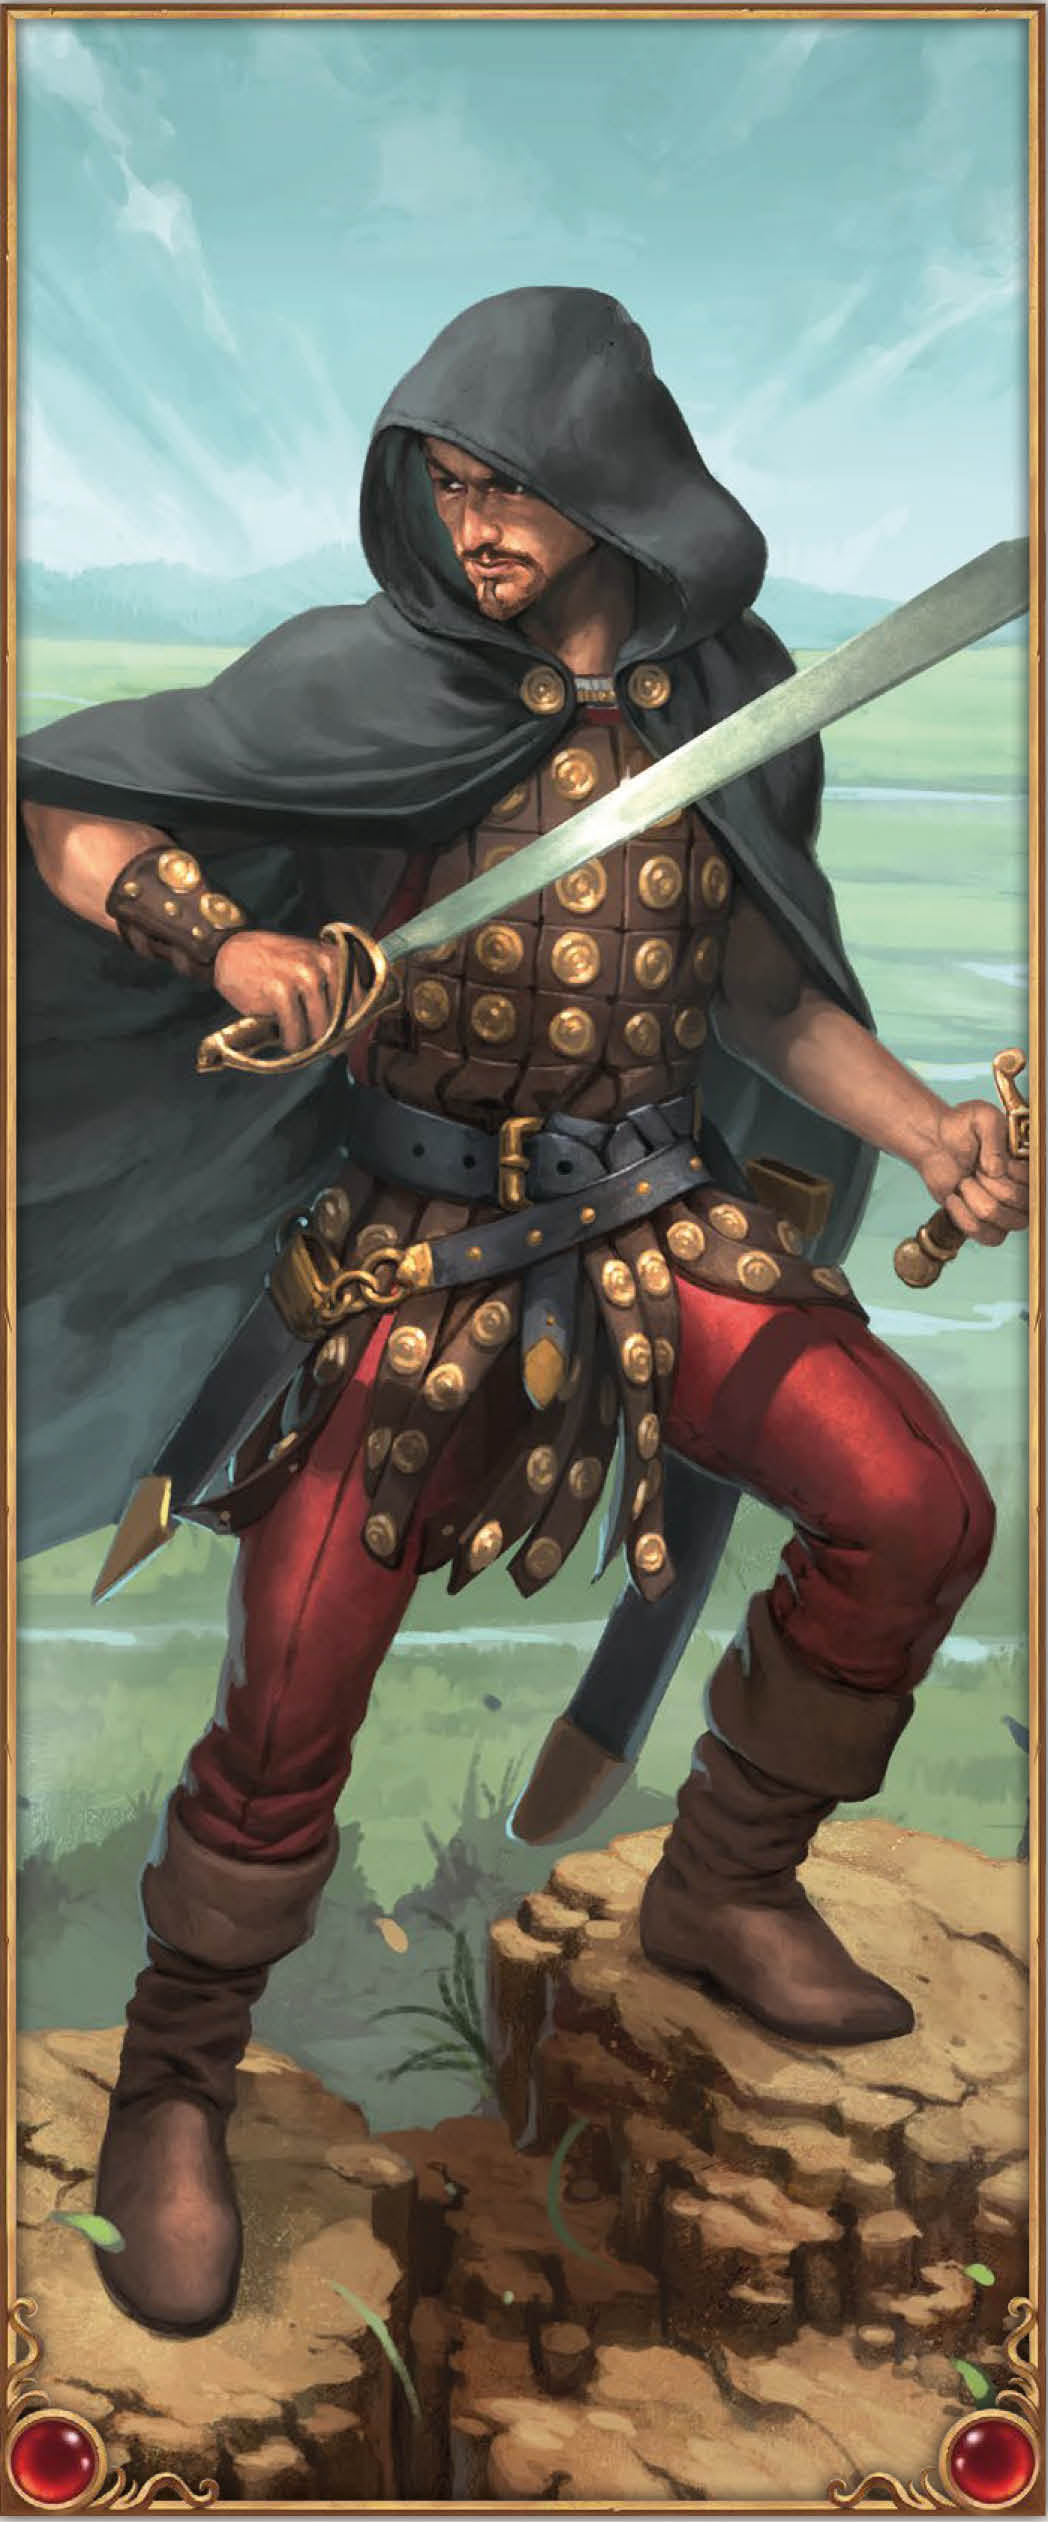
\includegraphics[width=\linewidth]{\art/rogue.jpg}

\subsection*{Combat with Neutral Units}

During combat with Neutral Units in clash sccenarios, if a player decides to deploy their Units only on one half (left or right one) of the battle board, the player positioning the Neutral Units must follow suit.

Placing Neutral Units far apart only makes the other player waste MPs, and that slows the game down.
The exception to this rule is when there are three Neutral \svg{unit_ground} Units to position, as all of them must go the front line.
See examples that follow.

\begin{center}
  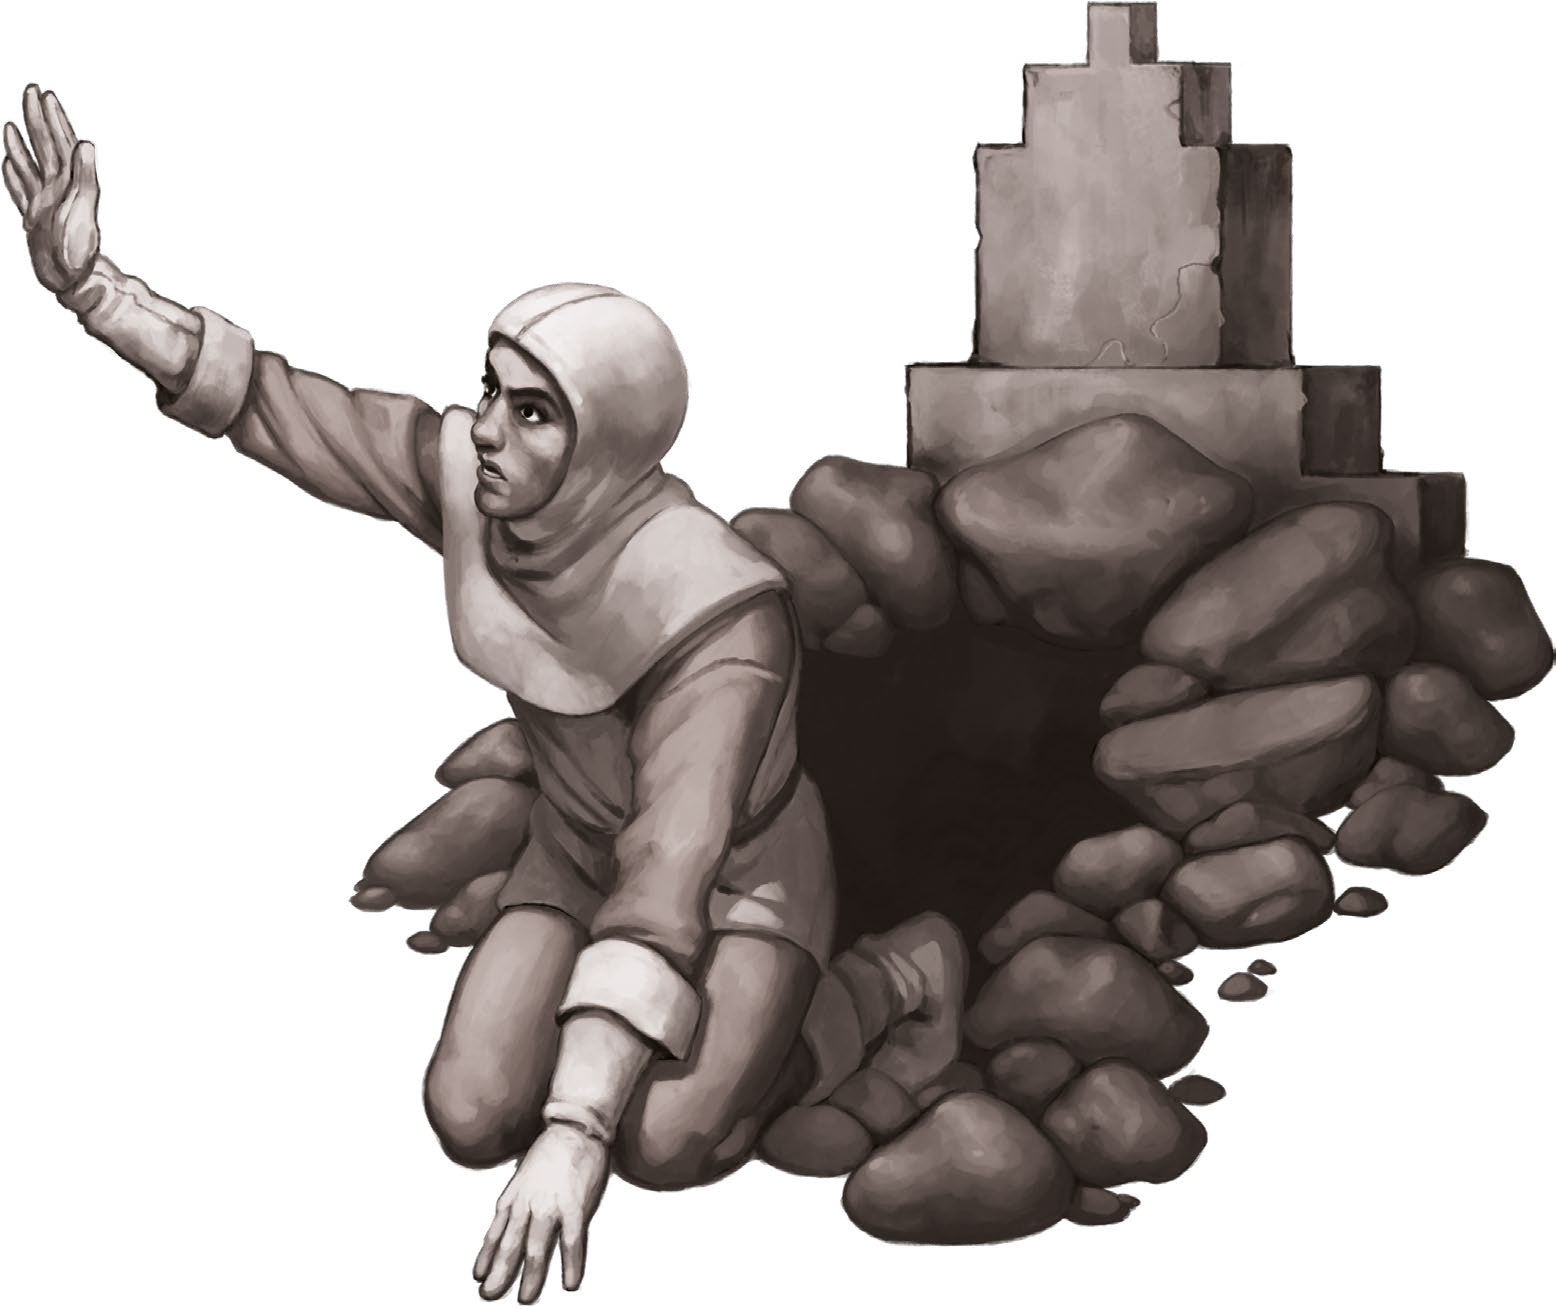
\includegraphics[width=0.65\linewidth]{\art/resurrection.png}
\end{center}

\end{multicols}

\begin{figure*}[!h]
  \mbox{}%
  \hfill%
  \begin{minipage}[t]{0.44\textwidth}
    \centering
    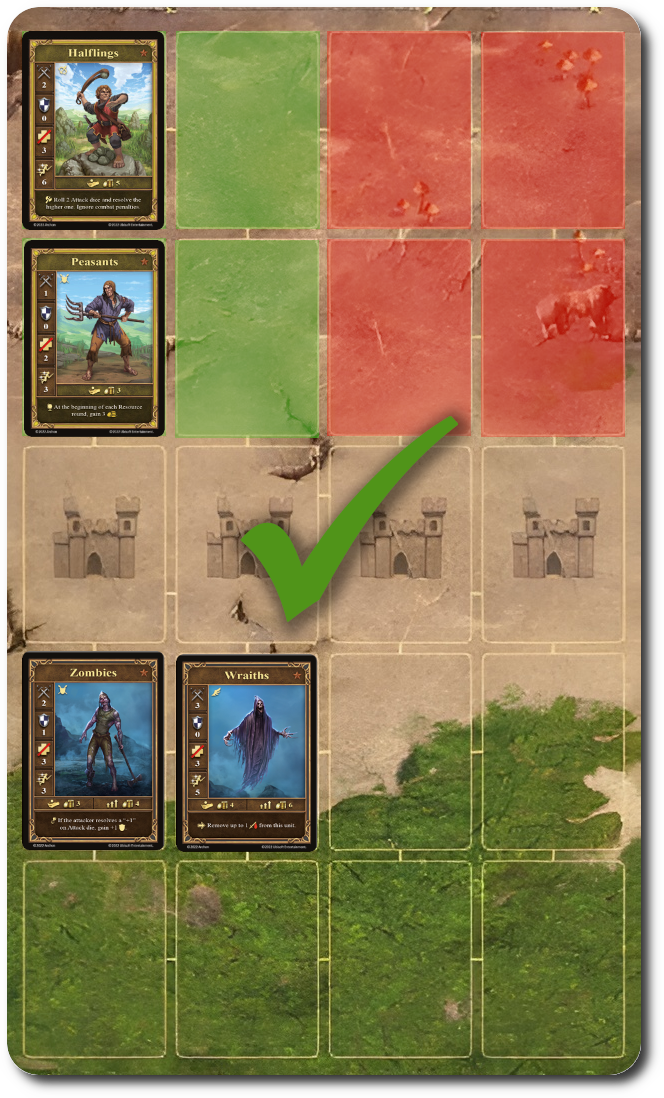
\includegraphics[width=\linewidth]{\examples/battle_good.png}
    \caption[good protected]{\textit{Neutral Units are positioned correctly.}}
  \end{minipage}
  \hfill%
  \begin{minipage}[t]{0.44\textwidth}
    \centering
    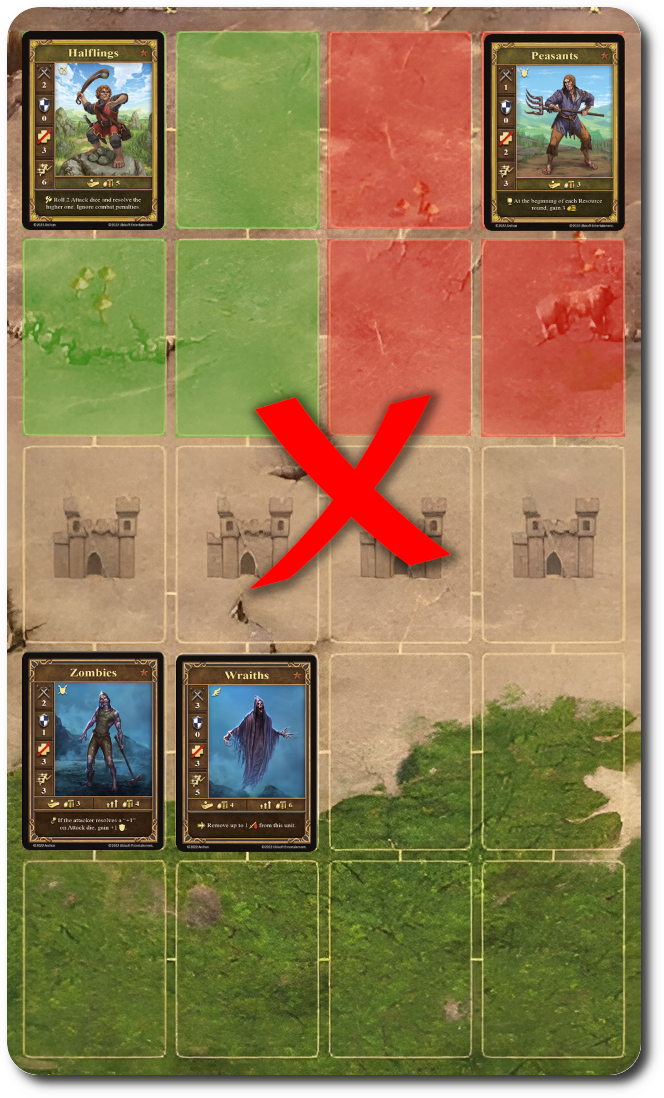
\includegraphics[width=\linewidth]{\examples/battle_bad.png}
    \caption[bad protected]{\textit{This is not allowed, as the Necropolis player deployd their Units on the left half of the Combat Board.
      The Peasants must start the Combat on the left side too.}}
  \end{minipage}
  \hfill%
  \mbox{}%
\end{figure*}

\clearpage

\begin{figure*}[!h]
  \mbox{}%
  \hfill%
  \begin{minipage}[t]{0.44\textwidth}
    \centering
    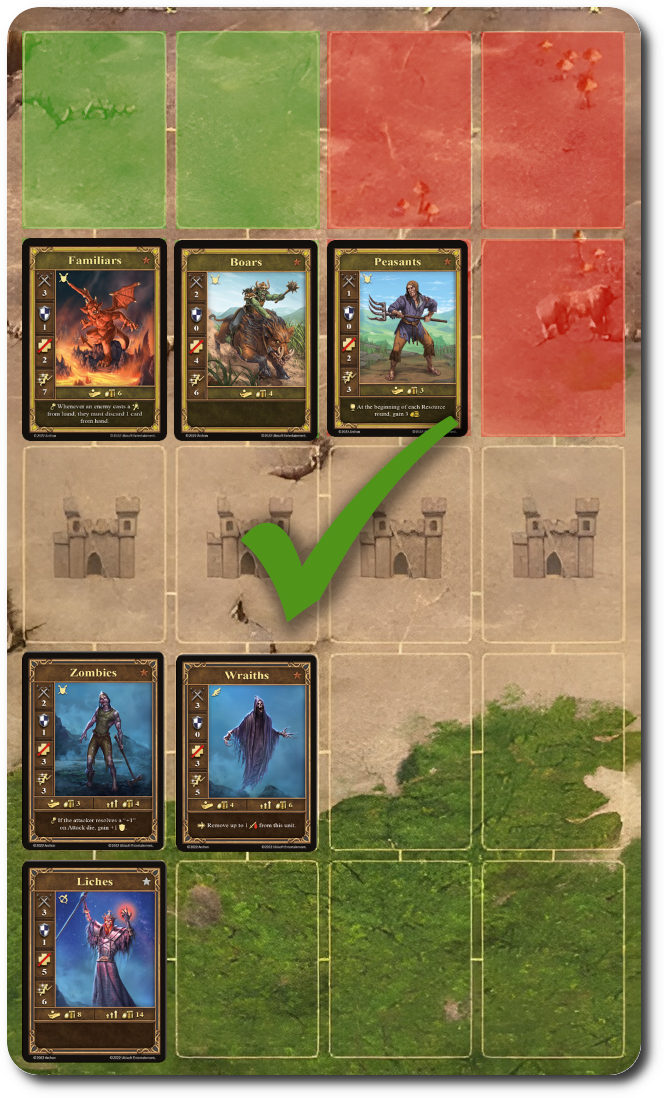
\includegraphics[width=\linewidth]{\examples/battle_exception.png}
    \caption[exception protected]{\textit{Exception: three \svg{unit_ground} Units must go to the front line.}}
  \end{minipage}
  \hfill%
  \begin{minipage}[t]{0.44\textwidth}
    \centering
    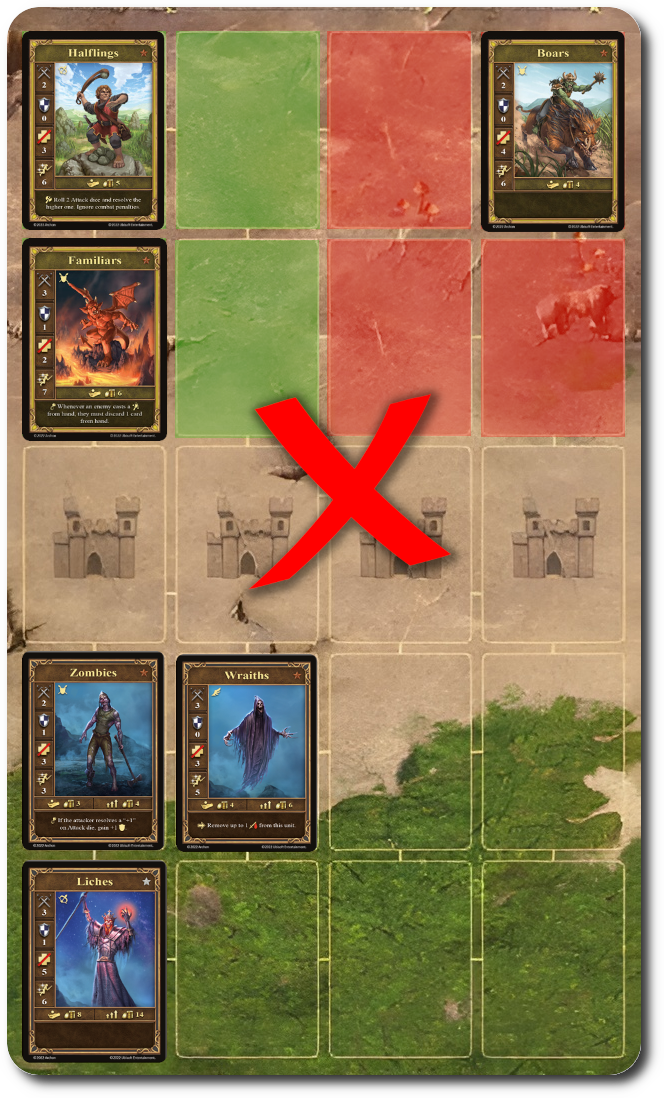
\includegraphics[width=\linewidth]{\examples/battle_ranged_bad.png}
    \caption[ranged protected]{\textit{The Boars must occupy one of the green fields.}}
  \end{minipage}
  \hfill%
  \mbox{}%
\end{figure*}

\begin{multicols}{2}

\subsection*{General Recommendations}

The following are not custom rules, but more like recommendations on how to get the most out of your game:
\begin{itemize}
  \item When deciding which building in your town to build, especially in the early game, it is \textit{usually} recommended to go for units, not city hall, mages guild or anything else faction-specific.
  \item If you struggle which spell, artifact or ability to pick, in general it's best to prioritize those that allow you to cycle through your deck.
    This means anything that can draw cards or pick cards from your discard pile.
  \item Try to limit spending the movement points of your main Hero on actions that the Secondary Hero can do, like flipping the Map tiles.
\end{itemize}

\begin{center}
  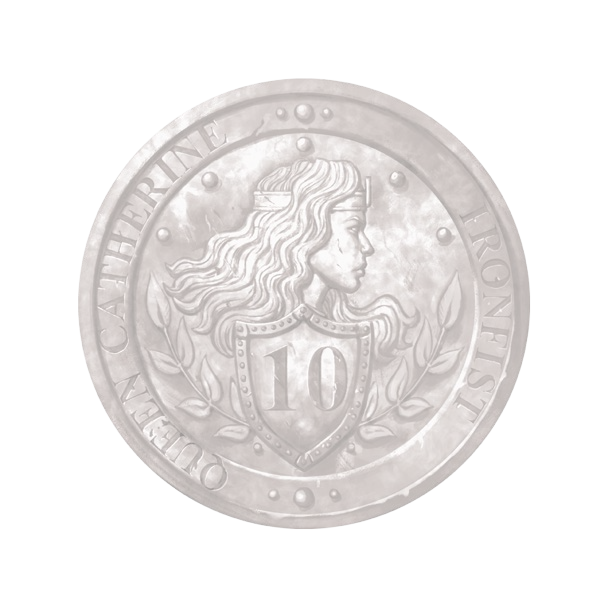
\includegraphics[width=0.7\linewidth]{\art/coin.png}
\end{center}

\end{multicols}
